\chapter{The Curious Asymmetry}

The US government currently consumes about 40\% of total GDP, when you consider
all the levels of government (local, state, and federal). The private sector is
regulated, but new businesses still sprout up and close down on a daily basis.
We are not close to anarchy and we are not close to communism.

In international comparisons, too often one sees the US Federal Government
compared with total government spending in other countries. This makes the US
seem like a small-government country. However, in the US system, state and
local governments spend too. Their share should count towards total government
spending.\footnote{It is also noteworthy that many other countries manage their
spending with a federal system or an even more local level, but that is rarely
mentioned in international comparisons. So, these comparisons really are apples
to oranges.}

If we look just at the economic role of government (which is the focus of this
book), we can place the possible governments from right to left. At one end of
the spectrum, we put the followers of Ayn Rand, exposing anarcho-capitalism:
there is no government or just a minimal government protecting private
property. At the other, we place full-blown communism with forced labor camps.
At the first end, individuals have all rights and there are no societal rights;
at the other end, individuals have no rights and society owns them as slaves.
Economically speaking, we are close to the middle of this spectrum.\footnote{On
non-economy dimensions, however, the 20th century has seen a steady walk from
the society to the individual end of the spectrum. I find it the most
surprising political fact of the last 100~years that the anarchists basically
won on state interference on sexuality. The result may not be the sexual utopia
that radical socialists predicted nor the Randian promise of a rational open
sexuality (her own real-life attempts were not as successful as those of the
characters in her novels). However, in policy, we live in anarchy. Despite the
fact that much hurt comes from it and that there is widespread condemnation of
adultery, it is a matter that has become a private and social matter, outside
the boundaries of courts.  This is, however, a topic for another book.} Still,
in polite speech there is too often an idea that we are on the verge of
political anarchy.\FIXME{Get quotes}

Yes, it is true that there are those that accuse Democrats of being Communists
or Nazis. A few signs in Tea Party demonstrations did compare Obama to Hitler.
However, this is not the establishment in the same way that op-eds in the New
York Times or University professors writing widely-read books. The fringe
libertarians (like the communists of 100 years ago), also enjoy their
infighting and are quick to term anyone who does not advocate
anarcho-capitalism as a statist.\footnote{A ``statist'' is someone who is not
against the state. This word is not even widely used, if at all, outside of the
anarchist millieux.} I'll still make the words of Scott Sumners
mine\backnote{On his blog, \emph{The Money Illusion},
\url{http://www.themoneyillusion.com/?p=23004}.\FIXME{Add full citation}}:

\begin{quote}
If one is a pragmatic libertarian, it is not inconsistent to argue the free
market is generally best, but also advocate patents, eminent domain, anti-trust
laws, low wage subsidies, the EPA and the Fed.  That still leaves plenty of
scope for free markets.  No country even comes close to having a government
that small.  That makes the term ``libertarian'' a useful description of the
person's policy views.
\end{quote}

One of the negative side-effects of this discourse is that it allows the
big-government GOP to grab the credit for being small-government, while never
really addressing any of the major interventions that the government has in the
economy. They consistently vote for major farm subsidies, a completely needless
(and costly) intervention in the economy.\footnote{The only element of the farm
bills that consistently gets cut with bipartisan support are the tiny part that
supports school lunches for children. The major cost of the bill comes, of
course, from subsidies to farmers in various guises.}\FIXME{find link to news
items.}


\section{Economic Freedom is Important}

In this book, I ask you to consider economic freedom as an important freedom.
Not all trumping, ``taxation is theft,'' kind of freedom; but something that we
need to respect and be careful when we abridge it. Consider the case of another
basic right, that of free-speech. I could make the following argument:

\begin{quote}
The idea that there is a free-speech right is an illusion. It might make us
feel good, but, upon further examination, we quickly detect the falsehood.
Historically, there has never been completely free speech. We cannot shout
``fire'' in a crowded movie theater and certain forms of obscenity have always
been banned.

Or consider the criminal master-mind who, upon getting arrested, claims that
``yes, he did say that so-and-so should be killed and even offered money for
it,'' but that is purely speech, he did not pull any triggers. Therefore, he
has a First Amendment Right to Free Speech and the charge of conspiracy is a
violation of his rights.

This is absurd. Society has an interest in what people say. Once you accept
this, you see that there is really no difference (except in degree) between
banning libel and banning criticism of elected officials.
\end{quote}

Naturally, we understand that the above argument is bunk. Accepting certain
restrictions to unbridled speech does not mean that there is no right to free
speech. It means that the free speech can only be regulated when equally
important rights are at stake. In institutional terms, this means that free
speech regulation has an extra layer of protection in the form of judicial
supervision that more run-of-the-mill legislation does not.

Valuing free speech does not mean that there are no limits to it, that does
limits cannot change in response to cultural changes (prohibitions on erotic
material are certainly much more relaxed than before), or that there can be
strong and vigorous disagreements on what is and is not an acceptable limit to
free speech (as the Supreme Court ruling in the Citizens United case on
campaign finance made clear, there is not even complete agreement as to what is
speech and what is not).

Yet, in the area of economic rights, too often, it seems that simply pointing
out that there are necessarily limits and have always been limits to economic
rights, means that the concept is meaningless. Instead, I think that we should
interpret the concept of economic rights like we interpret free speech:
violating those rights can be necessary, it can even be a good thing to do (if
it leads to a better society), but there should be a high level of scrutiny
and, unless there are strong arguments for the violation, we should preserve
people's rights.

Therefore, we can talk about economic rights and not necessarily defend Randian
anarcho-capitalism. Similarly, an argument that denies that these arguments are
absolute does not give the state full power to take someone's house and give it
to someone else because that person will pay more taxes.\footnote{In the US,
the government cannot take a single house, but it can take a whole neighborhood
and demolish it to give it to someone who will pay more taxes by declaring the
neighborhood as \emph{blighted}. Thus ruled the Supreme Court in \emph{Kelo vs.
City of New London}.}

\section{The Rabbit Curve}

This is the \emph{Rabbit Curve}:

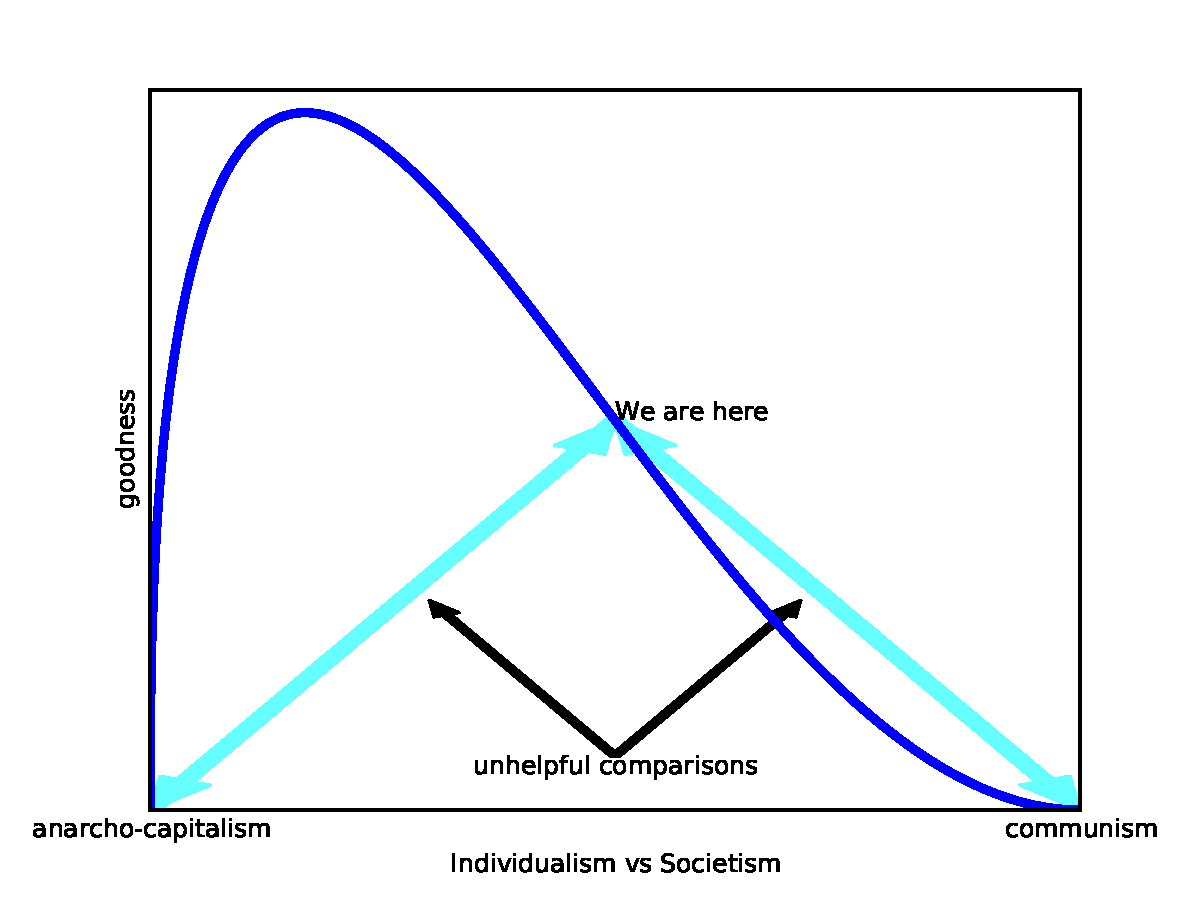
\includegraphics[width=.8\textwidth]{images/rabbit-curve.pdf}

It plots society rights vs.\ ``goodness.'' I could have written
\emph{efficiency} to make it sound more technical.

\subsection{Regulation is Necessary}



\subsection{Curious Asymmetry Thoughts}

\thought Socialism versus anarcho-capitalism is a false dichotomy. Neither is a
choice in front of us right now.

\thought Property rights are not absolute rights, but we still should be
careful not to trampled them for little gain.

\thought We are not on the verge of anarchy.

\thought If X is a problem, we have to address X; not regulate the whole
economy to prevent X from happening.

\thought Regulation vs.\ deregulation is (in the modern political economy)
rarely a useful frame of debate, misregulation is a much more common problem
than either.

